% ============================================================
% f2013_tianjin_science_q17_prism.tex
% 2013 天津卷（理科）第 17 题 四棱柱 ABCD-A1B1C1D1（TikZ 矢量重绘）
% 题设：A1A⊥底面 ABCD，AB∥DC，AB⊥AD，AD=CD=1，AA1=AB=2，
%       E 为 AA1 中点。底面为直角梯形，图中按斜二测投影绘制。
% 实线：可见棱；虚线：被遮挡棱与辅助线 AC、CE、EC1。
% ============================================================
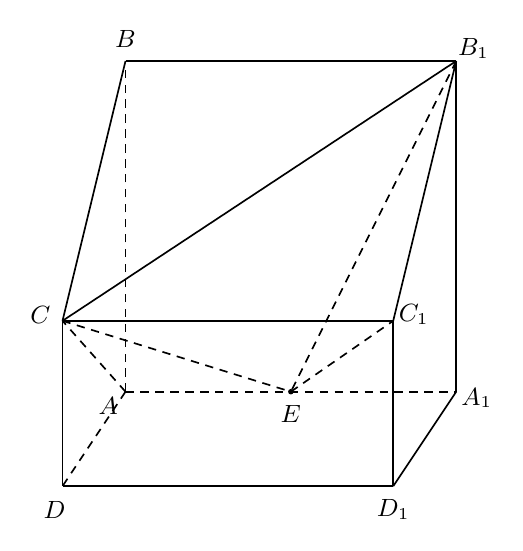
\begin{tikzpicture}[
  x=1cm, y=1cm,
  every node/.style={font=\small, inner sep=1pt},
  s/.style={line width=0.6pt},
  d/.style={line width=0.6pt, dash pattern=on 3.0pt off 2.4pt},
]

  % ---------- 实线 ----------
  \draw[s] (0,0) -- (0,2.10);          % D-C
  \draw[s] (0,2.10) -- (4.20,2.10);    % C-C1
  \draw[s] (4.20,2.10) -- (4.20,0);    % C1-D1
  \draw[s] (4.20,0) -- (0,0);          % D1-D

  \draw[s] (0,2.10) -- (0.80,5.40);    % C-B
  \draw[s] (0.80,5.40) -- (5.00,5.40); % B-B1
  \draw[s] (5.00,5.40) -- (4.20,2.10); % B1-C1
  \draw[s] (5.00,5.40) -- (5.00,1.20); % B1-A1
  \draw[s] (5.00,1.20) -- (4.20,0);    % A1-D1
  \draw[s] (5.00,5.40) -- (0,2.10);    % B1-C

  % ---------- 虚线 ----------
  \draw[d] (0.80,1.20) -- (0.80,5.40); % A-B
  \draw[d] (0.80,1.20) -- (0,0);       % A-D
  \draw[d] (0.80,1.20) -- (5.00,1.20); % A-A1（过 E）
  \draw[d] (0.80,1.20) -- (0,2.10);    % A-C
  \draw[d] (0,2.10) -- (2.90,1.20);    % C-E
  \draw[d] (2.90,1.20) -- (4.20,2.10); % E-C1
  \draw[d] (5.00,5.40) -- (2.90,1.20); % B1-E（原页辅助线）

  % E 点
  \fill (2.90,1.20) circle [radius=0.035];

  % ---------- 标签 ----------
  \node at (0.58,1.02) {$A$};
  \node at (0.80,5.68) {$B$};
  \node at (-0.28,2.18) {$C$};
  \node at (4.46,2.18) {$C_1$};
  \node at (-0.10,-0.30) {$D$};
  \node at (4.20,-0.30) {$D_1$};
  \node at (5.26,1.12) {$A_1$};
  \node at (5.22,5.56) {$B_1$};
  \node at (2.90,0.92) {$E$};

\end{tikzpicture}
